%%%%%%%%%%%%%%%%%%%%%%%%%%%%%%%%%%%%%%%%%%%%%%%%%%%
%
%  New template code for TAMU Theses and Dissertations starting Fall 2012.  
%  For more info about this template or the 
%  TAMU LaTeX User's Group, see http://www.howdy.me/.
%
%  Author: Wendy Lynn Turner 
%	 Version 1.0 
%  Last updated 8/5/2012
%
%%%%%%%%%%%%%%%%%%%%%%%%%%%%%%%%%%%%%%%%%%%%%%%%%%%

%%%%%%%%%%%%%%%%%%%%%%%%%%%%%%%%%%%%%%%%%%%%%%%%%%%%%%%%%%%%%%%%%%%%%%
%%                           SECTION I
%%%%%%%%%%%%%%%%%%%%%%%%%%%%%%%%%%%%%%%%%%%%%%%%%%%%%%%%%%%%%%%%%%%%%


\pagestyle{plain} % No headers, just page numbers
\pagenumbering{arabic} % Arabic numerals
\setcounter{page}{1}


% \renewcommand*{\thefootnote}{\fnsymbol{footnote}}
\chapter[\uppercase{Introduction}]{\uppercase{Introduction}}
% \symbolfootnote[1]{Reprinted with permission from ``Introduction: The Importance of Research'' by AUTHOR et al., 2015. The Astrophysical Journal, Volume XYZ, Issue X, article id. XY, XY pp., Copyright 20XX by the American Astronomical Society.} }
% \renewcommand*{\thefootnote}{\arabic{footnote}}
% \setcounter{footnote}{0}

This work is focused on how we may use upcoming large-area sky surveys to better understand galaxy clusters in a cosmological context. Therefore, it covers a broad range of topics from the galaxy clusters themselves, to planning and observations, cosmology, probability and statistics, numerical simulations, data reduction, and machine learning. The work presented in this thesis stands at the emerging intersection of data science and astronomy. Specifically we focus on how the Hobby Eberly Dark Energy Experiment (HETDEX; \citealt{Hill2008}) will contribute to the study of galaxy clusters in a cosmological context.

To begin, we introduce many of the basic concepts needed to understand the relevance of this work. While, this overview is certainly not comprehensive, it should provide the basic knowledge to follow the remaining discussion. The following two chapters constitute the bulk of our analysis, and can be thought of as a theoretical study and a practical test of the theory. We conclude with a look to the future, and how this work might be extended to other pressing issues in astronomy, today.

But first, we begin by discussing what clusters of galaxies are, how they are deeply related to the fundamental properties of the universe, and how we go about studying them. We provide a brief introduction, through example, to some of the key concepts of machine learning, and conclude with a discussion of the importance of this work to set the stage for the discussion to come.

\section{Galaxy Clusters}
Clusters of galaxies are the largest bound, highly over-dense, systems of galaxies which are held together by the cluster's own gravity. First recognized by 19th century astronomers, their place in astronomical canon was solidified when Edwin Hubble proofed their constituent nebulae where not bound to the Milky Way \citep{Hubble1926} but collections of stars similar to the Milky Way. Work to understand their nature and origin began in ernest when \cite{Hubble1931} used the virial theorem and the galaxy velocities in the centers of the Virgo \citep{Smith1936} and Coma \citep{Zwicky1933} clusters to derive their masses. The immense mass derived exceeded the total stellar mass contributed by all galaxies many times over. This lead Zwicky to theorize the existence of large amounts of non-luminous matter, and coining the term ``dark matter'' (DM), which we still use today.  

Some controversy surrounds what exactly constitutes a cluster. Traditionally, the richness \citep{Abell1958}, the number of galaxies above a certain brightness associated with the cluster, has defined the dividing line between rich clusters, and poor groups of galaxies. Clusters with a richness of 30 or more are traditionally referred to as clusters and those structures with richness between three and 30 are classified as groups. This definition is far from universal, and as such, in this work, we will not make such a distinction, any bound system of galaxies we refer to as a cluster.

\begin{figure}[ht]
	\begin{center}
		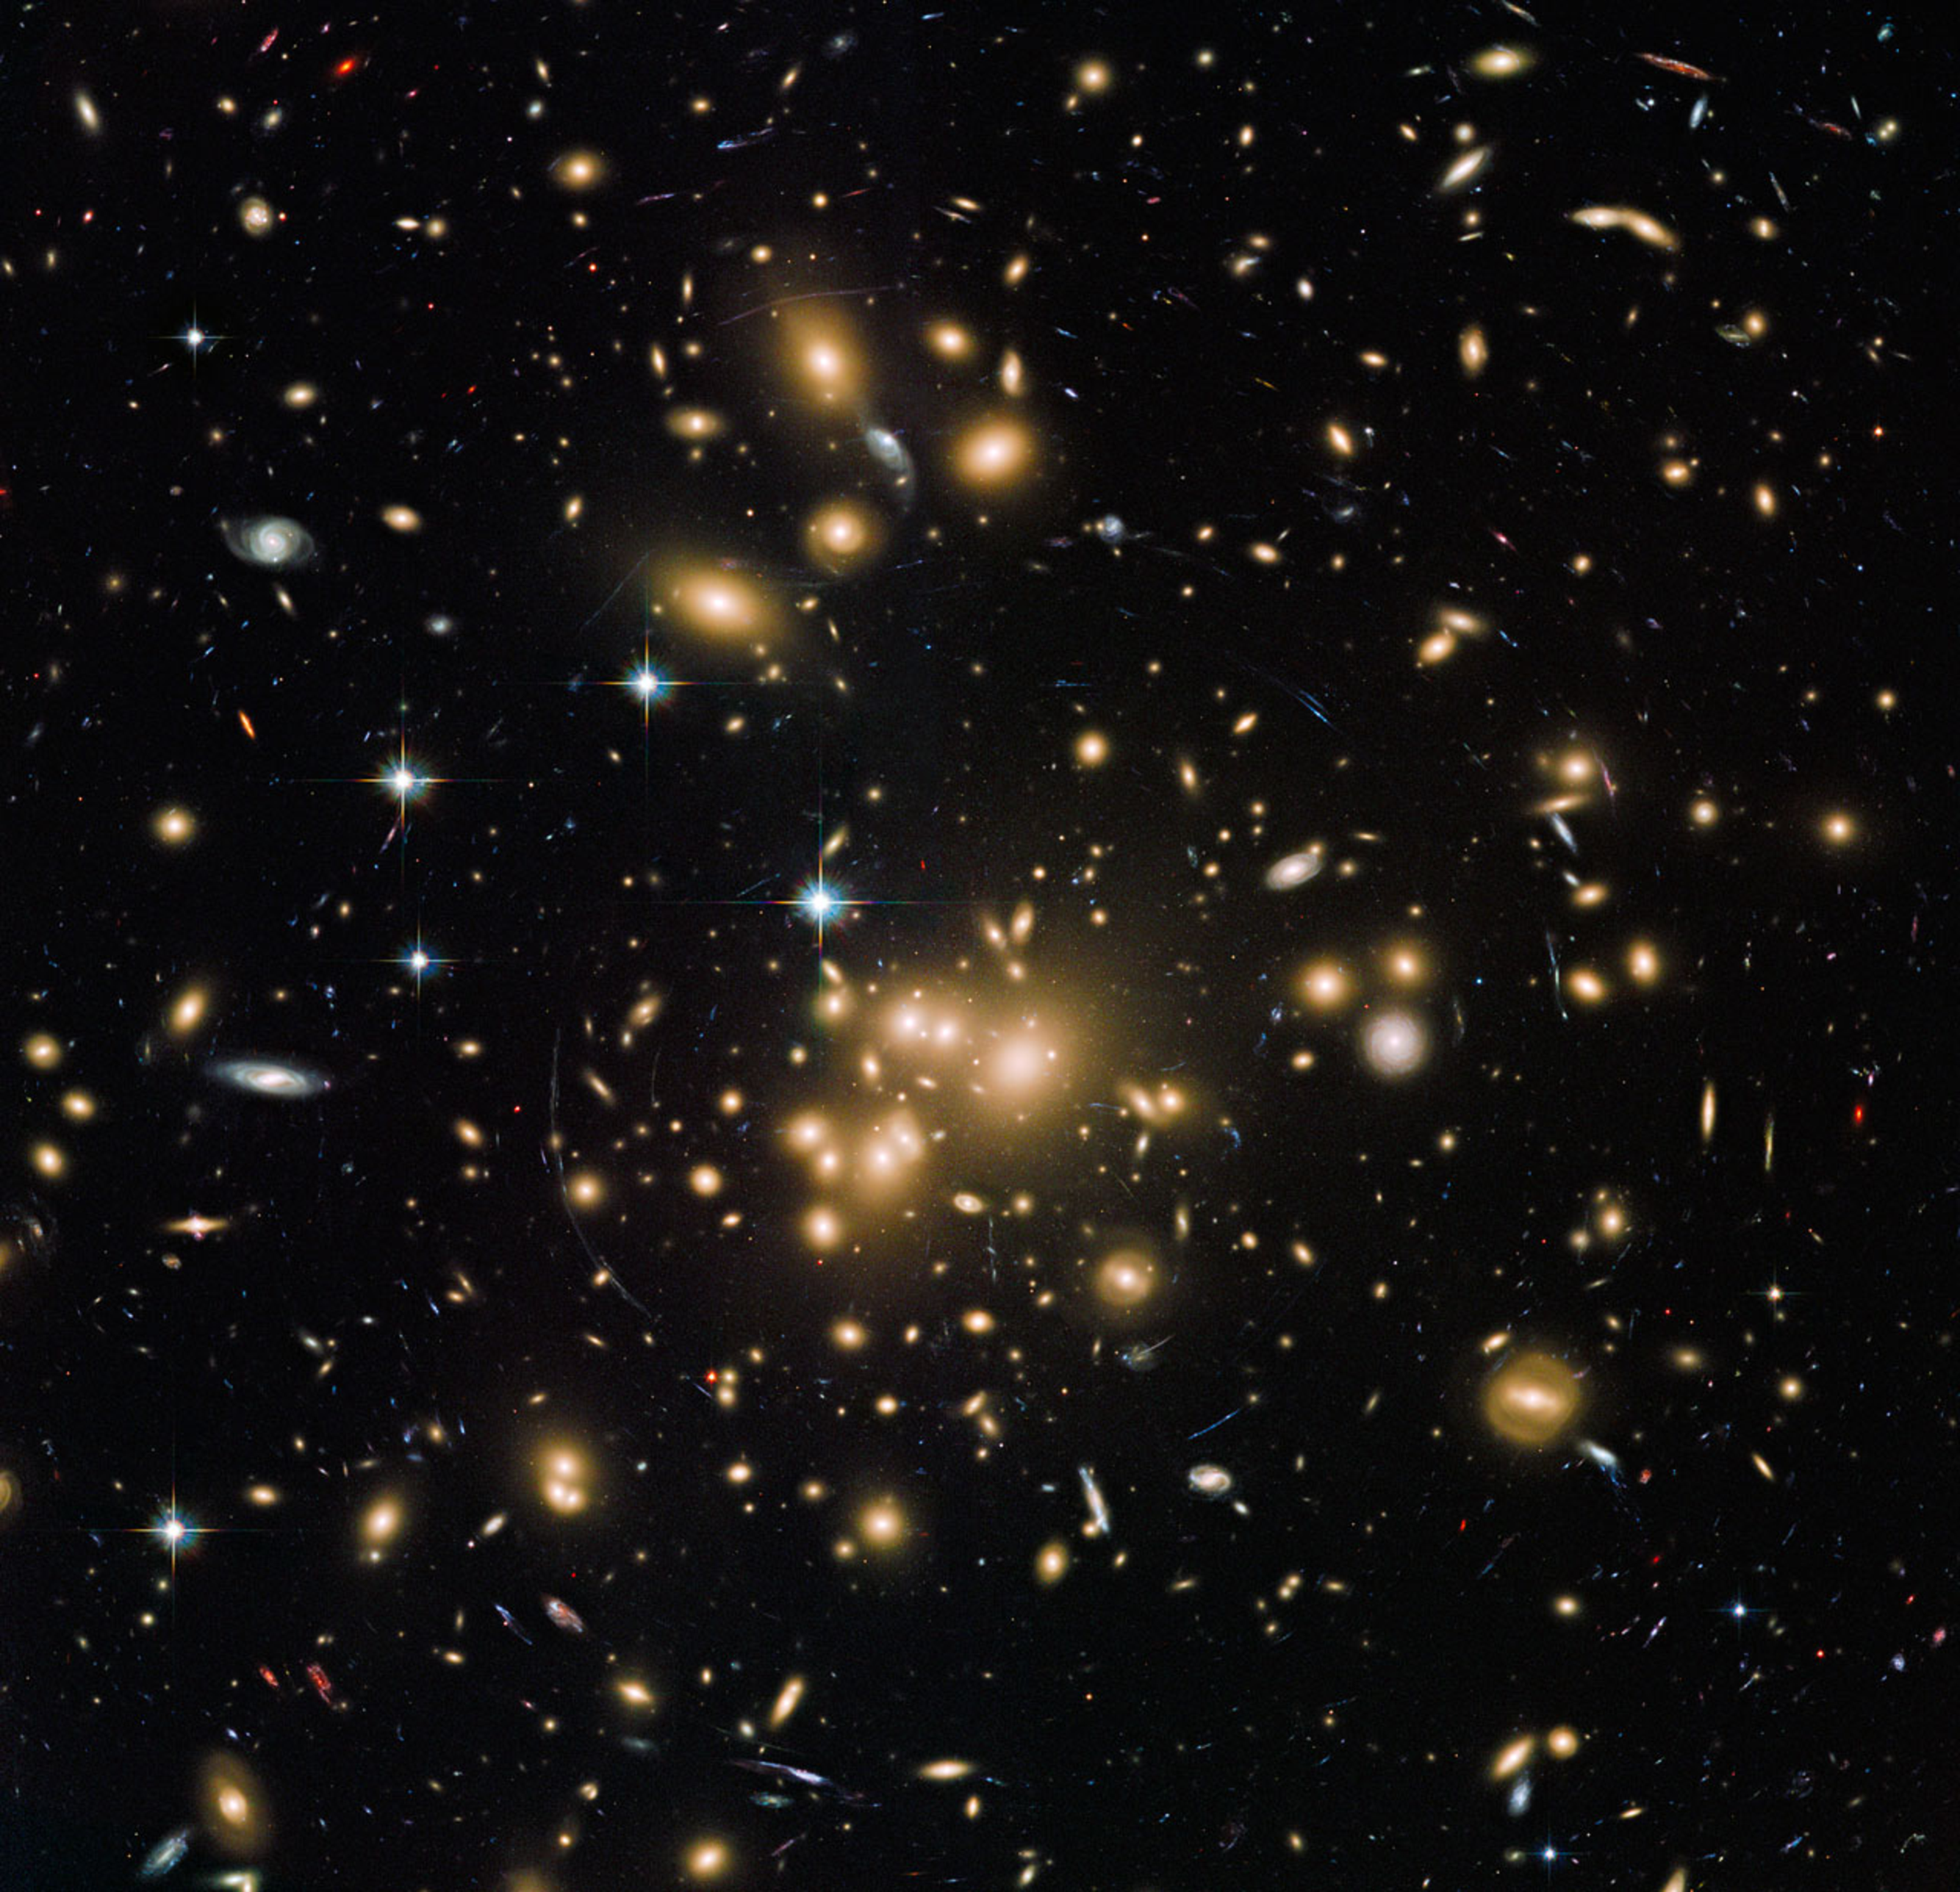
\includegraphics[width=0.6\textwidth]{figures/abell1689_hubble.pdf} 
	\end{center}
	\singlespace
	\caption{Hubble Space Telescope image of galaxy cluster Abell 1689.} Many of the galaxies visible are associated with the cluster. Not visible is the ICM or the larger DM halo which constitues the majority of the cluster mass.
	\label{fig: abell1689_hubble} 
\end{figure}

Modern astronomy gives the composition of galaxy clusters in three many parts. The galaxies themselves comprise the most obvious feature, and contain a large portion (but not the entirety) of the luminous matter (stars) in the cluster. The intracluster medium (ICM) is the space between the cluster galaxies and is composed many of ordinary matter (baryons) which are super heated to tens of thousands of kelvin. The ICM contains the bulk of the cluster's baryonic matter, and while it is very hot, it is not very dense, with a typical value of $10^{-3}$ particles per cubic centimeter. The majority of the cluster's mass is located in the DM halo which surrounds the cluster. For this reason, galaxy clusters are often referred to as halos, a term we use interchangeably throughout this work. Figure~\ref{fig: abell1689_hubble}\footnote{ESA/Hubble [CC BY 3.0 (http://creativecommons.org/licenses/by/3.0)]} shows a \emph{Hubble Space Telescope} Advanced Camera for Surveys image of galaxy cluster Abell 1689. Many of the cluster member galaxies have a similar yellow color. While the DM halo is not directly imaged, evidence for it can be seen by the very faint gravitational arcs of distant galaxies located behind the cluster.

Thought to form out of the primordial density fluctuations in the very early universe, the investigation of their formation and growth began in the 1960s. Soon thereafter, the hierarchical model of structure formation \citep{Press1974, Gott1975, White1978} was introduced. It suggests the first stars and stellar clumps grew then subsequently merged together with dark matter and other gas clumps to form the first galaxies which then continued to merge and grow into the clusters and large scale structures we see today. This accretion of smaller systems is thought to be driven by the gravity of the DM associated with the cluster. Of course, many complicated astrophysical processes are at work during cluster growth and similarly complicated theoretical models seek to explain these processes. For a detailed review of cluster formation see \cite{Kravtsov2012}.

Because their initial seeds were planted in the very early universe, the number and distribution of galaxy clusters across the sky is the finger print of the cosmology imprinted on the universe at its birth. To uncover the underlying cosmology a detailed understanding of the astrophysical processes that describe the motion of constituent galaxies and their impact on the ICM is required. So, galaxy clusters stand at the intersection of cosmology and astrophysics. 

\section{Cosmology with Galaxy Clusters}
The current concordance cosmology is a parametrization of the Big Bang cosmological model where the universe contains a cosmological constant ($\Lambda$; often referred to as dark energy) and cold dark matter (CDM). It is often characterized by six parameters; the Hubble Constant ($H_0$), the baryonic matter density ($\Omega_b$), the DM density ($\Omega_c$), the dark energy density ($\Omega_\Lambda$); the normalization of the power spectrum ($\sigma_8$); and the spectral index of the power spectrum ($n_s$). 

Galaxy clusters are sensitive probes of $\Omega_m$, the total mass ($\Omega_b + \Omega_c$) density in the universe and $\sigma_8$. Galaxy clusters trace the peaks in the universal matter density, often referred to as the power spectrum of matter density fluctuations or the matter power spectrum, much in the same way islands (mountain peaks) trace land masses through the ocean. We can constrain the values of $\Omega_m$ and $\sigma_8$ by comparing the number density of the observed galaxy clusters to that predicted by cosmological models.

The determination of cosmological parameters is done by comparing the number of galaxy clusters per unit mass per unit comoving volume ($n(M,z)$) to models. See \cite{Allen2011} for a comprehensive review or \cite{Murray2013} for a more practical approach. $n(M,z)$, referred to as the halo mass function (HMF) captures the number evolution through a function which defines the particular model used. Early work by \cite{Press1974} and \cite{Bond1991} which assumed spherically symmetric halos, have largely been replaced by more modern fitting functions which, at the expense of an analytical solution, provide more accurate results when fit to simulation data. See \cite{Murray2013} for a review of the most common fitting functions used. Through this approach, the two parameters which clusters are most sensitive to, $\Omega_m$ and $\sigma_8$, are in reality measured as $\sigma_8\Omega_m^\alpha$, where the value of $\alpha$ depends on the masses of the halos considered. The degeneracy is broken through the evolution of the HMF as a function of redshift. 

The accuracy of the estimates of $\Omega_m$ and $\sigma_8$ depends on how well the observed HMF can be measured. The correctness of the HMF depends directly on the number of galaxy clusters observed and the accuracy to which the mass of each of the clusters can be estimated. As we discuss below, the identification of large numbers of clusters is not a large contributing factor to the uncertainty; the total number of clusters known is only increasing. The accurate recovery of galaxy cluster mass for both very rich clusters (those with high mass) and, importantly, the poor clusters (those with low mass) remains the dominate source of uncertainty.

\section{Observations of Galaxy Clusters}
Observations of galaxy clusters span almost the entire electromagnetic spectrum, from the X-ray to the radio. For our purposes we focus on three which are most useful for estimating cluster mass. We discuss them in order of increasing wavelength.

\subsection{X-ray}
As mentioned previously, the majority of a galaxy cluster's baryonic matter is located in the hot ICM. The gas which makes up the ICM is falling into the gravitational potential well of the cluster, and is heated to tens of megakelvins. Such high temperatures causes the gas to emit X-rays through the bremsstrahlung process. The X-ray luminosity ($L_X$) of a galaxy cluster correlates with the depth of the gravitational potential well, which leads to an estimate of the cluster's mass \citeeg{Finoguenov2001}. 

The $L_X$ of a cluster is a relatively easy measurement, requiring only a few photons to measure. However, at fixed cluster mass $L_X$ decreases quickly with increasing redshift, which limits X-ray selected samples of galaxy clusters to redshifts $< 1$. X-ray identified clusters, up until today, have mostly been observed purposefully through targeted \textit{Chandra} or \textit{XMM-Newton} observations. That is soon to change with the \textit{eROSITA} \citep{Pillepich2012} telescope onboard the Spektrum-Roentgen-Gamma Mission, which will perform an all-sky survey during its four year mission and detect an estimated 50,000 or more clusters.

\subsection{Optical}
To determine which galaxies do and not belong to a given cluster, optical observations play a key role. This makes it possible to identify and study individual galaxies in a cluster environment, but it can also provide an estimate of the cluster's total mass. Much like the X-ray observations the motions of the individual member galaxies (called a velocity dispersion) provides an estimate of the depth of the cluster's gravitational potential well, which is an estimate of the total cluster mass. The constituent cluster galaxies act as tracer particles through the cluster's potential well, which can be modeled in simulations and has been the focus of many recent studies \citeeg{Evrard2008, Saro2013, Sifon2013, VanderBurg2014, Munari2015}. This type of measurement is important because it is independent of the physics of the ICM, which are not fully understood. However, this type of measurement requires spectroscopy, which is expensive to obtain. 

\begin{figure}[ht]
	\begin{center}
		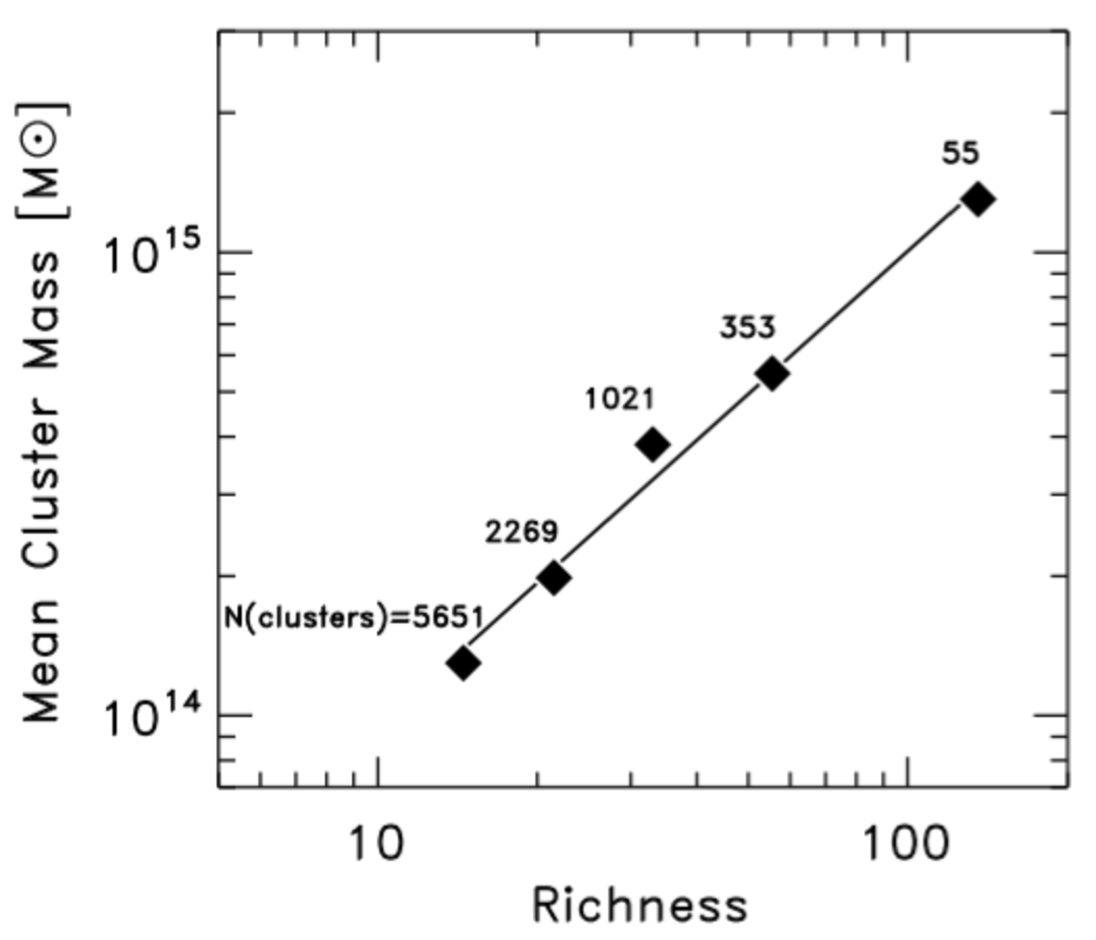
\includegraphics[width=0.6\textwidth]{figures/massrichness.pdf}
	\end{center}
	\caption{The relation between the mean Richness and the mean cluster mass.} 
	Derived from stacked weak lensing measurements and adapted from \citealt{Rozo2010}, the number of clusters in each stack are given above each data point. There is a strong correlation between richness and cluster mass, however, because the data are stacked, the absolute mass scale and scatter in mass at fixed richness are imprecisely known.
	\label{fig:massrichness}
\end{figure}

It is possible to estimate both cluster membership and mass through photometric observations alone. Modern cluster finding algorithms such as the red-sequence Matched-Filter Probabilistic Percolation (redMaPPer; \citealt{Rykoff2014}) which measures a galaxy cluster's richness. The richness measurement, in the case of redMapper, is a probability weighted cluster membership, where the probability is whether or not an individual galaxy belongs to the cluster in question. Figure~\ref{fig:massrichness} shows the richness correlates strongly with cluster mass on average \citeeg{Rozo2010}, but the absolute mass scale of the optical richness mass estimator and the scatter in cluster mass at fixed optical richness are imprecisely known \citep{Rykoff2012}.

Large optical surveys such as the Dark Energy Survey (DES; \citealt{DES2005}) and the Large Synoptic Survey Telescope (LSST) will survey enormous portions of the sky extremely deeply and will identify vast numbers of clusters using optical selection methods \citeeg{Rykoff2014, Rozo2014}. However, the majority of these surveys will be photometric, and any spectral information will be obtained from preexisting datasets. And while it is possible to estimate cluster masses using photometric redshifts, primarily through the richness-mass relation, spectroscopic followup is required to both better calibrate the relation and to obtain the level of precision needed to compete with other mass estimators. 

\subsection{The Sunyaev-Zel'dovich Effect}
Millimeterwave observations of the Cosmic Microwave Background radiation (CMB) can show the presence of galaxy clusters. Through an effect called the (thermal) Sunyaev-Zel'dovich effect (SZE; \citealt{Sunyaev1972}) which is the up-scattering of CMB photons as they pass through the hot ICM. Through inverse Compton scattering, the CMB photons receive an energy boost when they collide with the high energy electrons of the ICM. This energy boost leads to a minor blue-shift of the CMB spectrum. This effect is illustrated in Figure~\ref{fig:sze}. 
\begin{figure}[ht]
	\begin{center}
		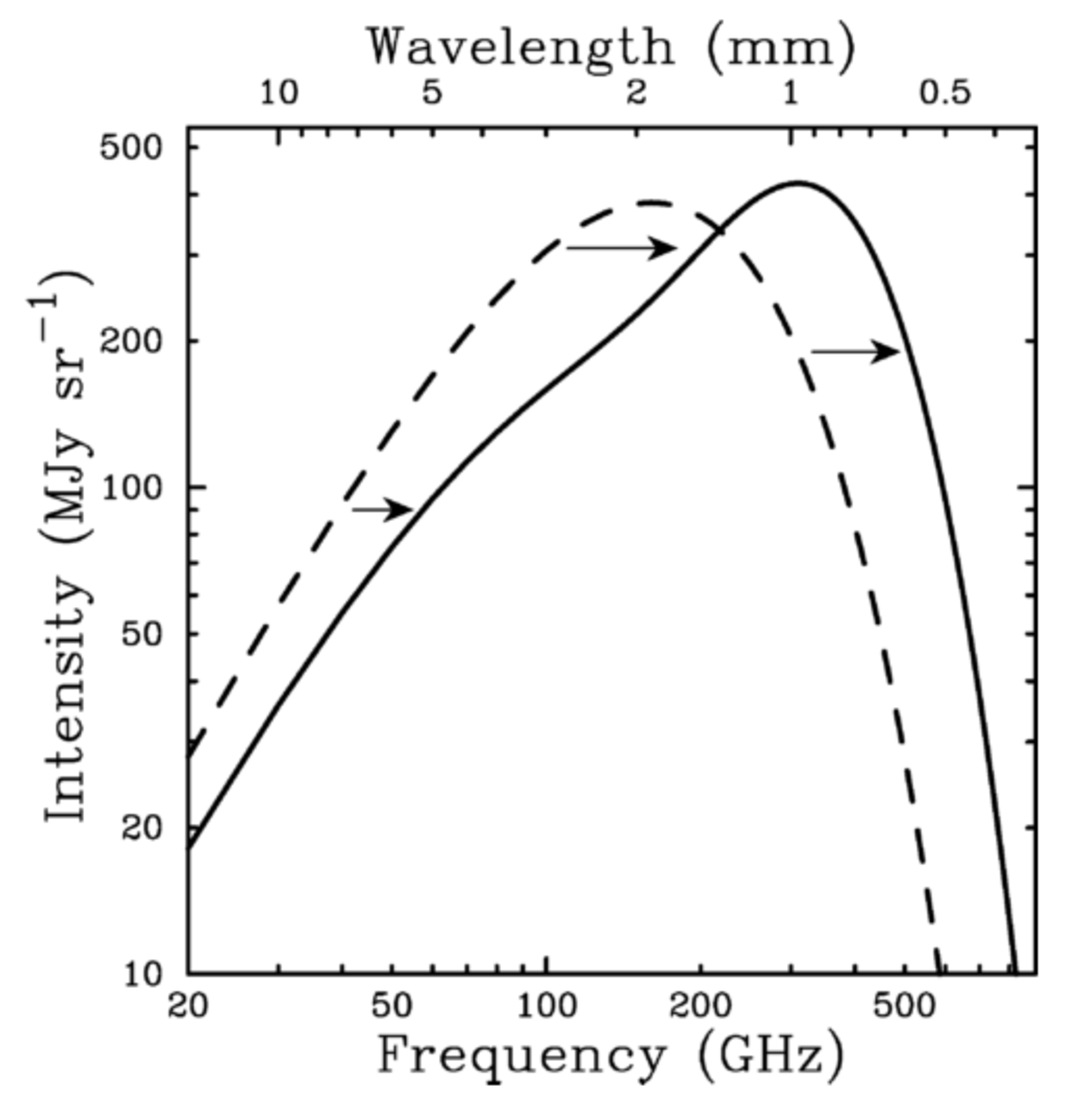
\includegraphics[width=0.6\textwidth]{figures/sze.pdf}
	\end{center}
	\caption{The Sunyaev-Zel'dovich Effect.}
	Adapted from \cite{Carlstrom2002a}, the undistorted CMB spectrum (dashed line) is shifted to a higher energy (solid line) by the SZE. Note: this shift is for illustration purposes only, the SZE distortion shown is for a fictional cluster 1000 times more massive than a typical massive galaxy cluster.
	\label{fig:sze}
\end{figure}
High resolution images of the CMB can detect a ``hole'' in the CMB at frequencies below 218 GHz, and a bright spot at higher frequencies, due to the shift in the CMB black body spectrum. The temperature of the ICM effects the depth (or height) of the CMB observations, which similarly to the X-ray observations, provides an estimate of the cluster's total mass. 

At their completion, the South Pole Telescope (SPT; \citealt{Carlstrom2011}) and the Atacama Cosmology Telescope (ACT; \citealt{Swetz2011}) are expected to find approximately one thousand clusters using observations in the millimeter combined with the SZE. Attempts are already underway to calibrate these observations using subsamples of clusters (approximately 100 cluster candidates and 60 clusters respectively) and other observables such as optically-based, virial estimates or X-ray temperature measurements \citeeg{Sifon2013, Bocquet2015}. 

\section{Galaxy Cluster Surveys as a Data Science Challenge}
Astronomy and astrophysics are undergoing a data revolution. The advances in telescope design, detectors, and computing resources have provided more astronomical data than any previous time in the history of the field. Beginning in the early 2000s, astronomical surveys have generated many hundreds of terabytes of data for many millions of sources. In the coming years, this data excess will grow beyond the terabyte regime with observations of billions of astronomical objects. 

50,000 or more X-ray identified clusters will be found by the upcoming eROSITA telescope onboard the \emph{Spektrum-Roentgen-Gamma} Mission. SPT and ACT are discovering many thousands of clusters through the SZE. DES and LSST will optically identify \citeeg{Rykoff2014} many tens of thousands of clusters with much lower masses than is possible with SZE measurements. The data products from these surveys will be both immense and heterogeneous. The number of observational parameters associated with each cluster can be many tens. The different observation wavelengths probe different cluster physics making them more or less sensitive probes of a specific galaxy cluster's total mass. The instruments used to collect the data have varying angular resolutions, owing from both the wavelengths observed and ground versus space based observations. The combination of datasets will be a significant challenge.

The ability to associate individual or combinations of observations with the cluster property in question will be a powerful statistical tool. Combining redshift with velocity dispersion measurements could potentially produce more accurate estimates of cluster mass with smaller scatter. However, the process by which the observations are combined is not a trivial exercise. Machine learning offers a promising approach.

\subsection{Machine Learning}
Machine learning (ML) is a branch of computer science focused on the study and construction of computational tools which can learn from and make predictions based on data. In 1959, Arthur Samuel (December 5, 1901 -- July 29, 1990), an early computer gaming pioneer, described ML as a ``Field of study that gives computers the ability to learn without being explicitly programmed.'' While, a great deal of programming is often required (discussed further below), such algorithms work by comparing data to a set of models allowing them to make predictions based on the data rather than preprogrammed commands.

ML can be broken into two large categories. ``Unsupervised learning'' where the ML is tasked to make qualitative statements about the data which were not previously known. An example would be finding clusters of data inside a large dataset, where the number and location of the clusters are not known a priori (\eg, locating galaxy clusters in observations of galaxy positions). ``Supervised learning'' asks the computer to make predictive statements about one variable based on the observations of another or combination of variables. An example could be photometric redshift prediction. Given a large number of color and magnitude measurements for a galaxy, predict the most probable redshift.  

In this work, we are concerned with supervised learning, where we know a relationship exists between two sets of data, and we use a computer algorithm to infer the relationship for us. To do this learning, we use an algorithm called decision tree learning which works by mapping a set of observations (``features'' in ML speak) of an source to a set of conclusions (``targets'') about that source. If the set of conclusions is finite then the method becomes a classification tree, and if the conclusions infinite then it becomes a regression tree. 

\begin{figure}[ht]
	\begin{center}
		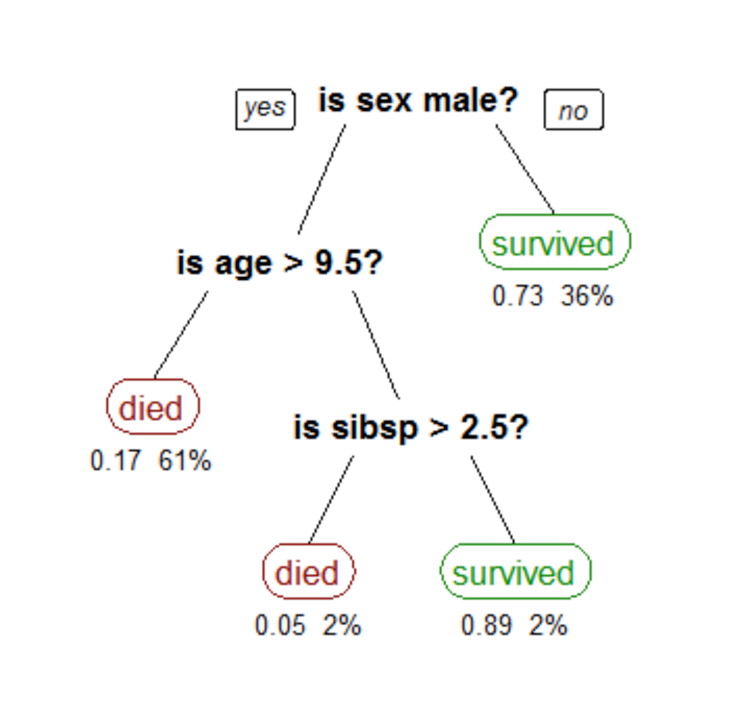
\includegraphics[width=0.6\textwidth]{figures/CART_tree_titanic_survivors.pdf} 
	\end{center}
	\caption{An example of a classification tree.}
	Decision tree classifying the survival of passengers on the RMS Titanic. ``sibsp'' represents the number siblings or spouses aboard, and the numbers below each class represents the probability of survival and fraction of passengers which are classified into each leaf. 
	\label{fig: cart tree} 
\end{figure}

Figure~\ref{fig: cart tree}\footnote{By Stephen Milborrow (Own work) [CC BY-SA 3.0 (http://creativecommons.org/licenses/by-sa/3.0) or GFDL (http://www.gnu.org/copyleft/fdl.html)]} shows a simple example of a classification tree for the survivability of passengers on the RMS Titanic. The bolded text are referred to as interior nodes which correspond to a single feature of each passenger in the example, sex, age and number of siblings or spouses. The ending points are called leaves which represents the value of the target variable given the value of the features input into the tree. For this example, there are two possible ending leaves, ``died'' or ``survived.'' Using this simple tree we are able to classify all passangers into the two possible classes. 

The ML algorithm ``learns'' this tree by choosing a feature from all available features which best splits the input data into two or more subsets. In the case of the example this is the sex of the passenger. This becomes the root node. All subsequent nodes are created by repeating this process on each subset associated with the previous node. So, it will split the male passengers by age, and then by number of siblings for the males older than 9.5 years. This process is known as a top-down induction of decision trees and is the most common method for creating decision trees from data.

Once the decision tree has been learned it can be used to classify data it has not seen before. For example, a 30 year-old, male passenger of the RMS Titanic has a probability of survival of 17\% and so will most likely be classified as ``died'' by the ML algorithm. However, imagine for a moment, with the benefit of hindsight that we know this male passenger survives. Only 17\% of the time will the ML method classify the passneger as ``survived'' based on this decision tree. We can boost the predictive power of the tree by generating many trees, and then combining the final predictions at the end. Methods that construct more than one tree are called ensemble methods. For this work, we use an ensemble method know as a forest of randomized trees, and discuss them more in Sections \editorial{XXXX}.

\section{This Work}
The goal of this work is to understand how a survey such as HETDEX can reduce the associated systematics of galaxy cluster mass scaling relations, specific the optical richness-mass scaling relation. HETDEX is a forthcoming blind spectroscopic survey that could potentially be used to accurately calibrate the richness-mass relation for a significant number of galaxy clusters at both extremes of the mass scale. The primary science mission for HETDEX is to measure the dark energy equation of state at $z\sim2$, and so the applicability to galaxy cluster science has not yet been investigated.

In this thesis, we first use a set of state-of-the-art simulations where we simulate the observing strategy of HETDEX to determine the number and nature of clusters that might be observed. This is accomplished in two ways, and in each part we measure the dynamical properties, such as redshift, velocity dispersion, and mass of the clusters. First we use targeted observations and perfect knowledge of the observed galaxy clusters, which includes center, membership, and number to recover the desired properties. Secondly, we assume that we know the location but not the center, membership, or number of constituent galaxies. Then we will employ the HETDEX observing strategy, including realistic pointing pattern, observational magnitude constraints, and spectral sensitivity limits to generate a set of realistic observations.

For the two sets of observations, we use three methods to estimate each galaxy cluster's mass, a traditional power law method, a probability based method, and a ML based approach. Then, using those cluster mass estimates we attempt to characterize the richness-mass relation (or relations) to better understand the dominate sources of uncertainty when using HETDEX like observations. This will enable us to more fully understand and constrain the HMF which, in turns, allows us to make more accurate measurements of the cosmological parameters traced by galaxy clusters.

As a practical test of the approaches we develop in the theoretical portion of this work, we use targeted spectroscopic observations of ten nearby clusters with the Mitchell Spectrograph (formerly known as VIRUS-P; \citealt{Hill2008a}), the prototype instrument for HETDEX, to estimate cluster properties. After determining cluster membership and applying many of the same cluster mass estimators as before, we again attempt to estimate the scatter and absolute scale of the optical richness-mass relationship.
